% Kompilacja: XeLaTeX (w Overleaf: Menu -> Compiler -> XeLaTeX).
% Do kompilacji potrzebny jest też katalog KM1 z ilustracją preprocessing_examples.png.
\documentclass[11pt,a4paper]{article}

\usepackage{fontspec}
\setmainfont{Latin Modern Roman}
\usepackage{polyglossia}
\setdefaultlanguage{polish}
\usepackage[margin=2.2cm]{geometry}
\usepackage{microtype}
\usepackage{booktabs,tabularx,array}
\usepackage{enumitem}
\usepackage{graphicx}
\graphicspath{{Results/KM1/}{KM1/}}
\usepackage[hidelinks]{hyperref}

\hypersetup{
  pdftitle={Kamień milowy 1 — Segmentacja obszaru odczytu wodomierza},
  pdfauthor={Wojciech Szewczyk},
  pdflang={pl-PL}
}
\setlength{\parindent}{0pt}
\setlength{\parskip}{5pt}
\setlist[itemize]{leftmargin=*,itemsep=2pt,topsep=3pt}
\setlist[enumerate]{leftmargin=*,itemsep=3pt,topsep=3pt}
\newcolumntype{Y}{>{\raggedright\arraybackslash}X}
\emergencystretch=1em

\begin{document}

\begin{center}
  {\Large\bfseries Segmentacja obszaru odczytu wodomierza\par}
  \vspace{4pt}
  {\large Kamień milowy 1\par}
  Definicja problemu, dobór danych i projekt eksperymentu\par
  \vspace{5pt}
  Wojciech Szewczyk
\end{center}

\section{Cel i zakres projektu}

Celem projektu jest automatyczne wskazanie obszaru z~cyframi na zdjęciu
wodomierza. Zadanie ma postać segmentacji binarnej: każdy piksel obrazu
jest przypisywany do obszaru odczytu albo do tła. Wynikiem działania modelu
jest maska pokazująca położenie tego obszaru.

Takie rozwiązanie może przygotowywać zdjęcia do automatycznego odczytu
zużycia wody. Projekt obejmuje lokalizację obszaru odczytu, bez rozpoznawania
cyfr. Główne pytanie badawcze brzmi:
\textbf{czy augmentacja danych poprawia jakość segmentacji w~porównaniu
z~uczeniem tej samej sieci bez augmentacji?}

\section{Zbiór danych i jego przygotowanie}

W~projekcie wykorzystano zbiór \textit{Water Meters Dataset}, udostępniony
w~serwisie Kaggle przez użytkownika tapakah68.\footnote{Źródło danych:
\url{https://www.kaggle.com/datasets/tapakah68/yandextoloka-water-meters-dataset}.}
Zestaw zawiera 1244 kolorowe zdjęcia JPG i~1244 odpowiadające im maski.
Szerokości obrazów źródłowych wynoszą 864--2058~px, a~wysokości 480--2168~px.

Zbiór odpowiada bezpośrednio wybranemu zadaniu i~zawiera gotowe oznaczenia,
dzięki czemu umożliwia zarówno uczenie nadzorowane, jak i~ilościową ocenę
predykcji. Zdjęcia różnią się rozmiarem, oświetleniem i~ustawieniem wodomierza.
Istotnym utrudnieniem jest mały udział obszaru odczytu: po preprocessingu
97,69\% pikseli masek stanowi tło. Sama dokładność pikselowa może więc
dawać myląco dobry wynik nawet przy słabej segmentacji.

Przygotowanie danych obejmuje skalowanie obrazów do $512\times512$ pikseli,
przeliczenie wartości do zakresu $[0,1]$, rozciąganie kontrastu na podstawie
2. i~98. percentyla oraz filtr medianowy $3\times3$. Maski są binaryzowane
przy progu 127 i~skalowane metodą najbliższego sąsiada.

W~projekcie rozróżniono \textbf{podstawowy preprocessing}, wspólny dla
wszystkich podzbiorów, oraz \textbf{losową augmentację}, która urozmaica
przykłady podczas treningu. Augmentacja nie jest warunkiem gotowości zbioru:
jest elementem porównywanych wariantów uczenia. Zbiory walidacyjny i~testowy
podlegają wyłącznie podstawowemu preprocessingowi.

Finalny podział utworzono z~ziarnem 42. Zbiór treningowy służy do uczenia
wag, walidacyjny do wyboru checkpointu i~wariantu, a~testowy do końcowej
oceny. Udziały klas obliczono z~masek po skalowaniu do $512\times512$:

\begin{center}
\begin{tabular}{lrrrr}
\toprule
\textbf{Zbiór} & \textbf{Pary} & \textbf{Udział zbioru} & \textbf{Obszar odczytu} & \textbf{Tło} \\
\midrule
Train & 995 & 79,98\% & 2,31\% & 97,69\% \\
Val & 124 & 9,97\% & 2,30\% & 97,70\% \\
Test & 125 & 10,05\% & 2,37\% & 97,63\% \\
\midrule
Łącznie & 1244 & 100,00\% & 2,31\% & 97,69\% \\
\bottomrule
\end{tabular}
\end{center}

Pary zapisano w~katalogach train/val/test. Podzbiory są rozłączne po nazwach
plików; kontrola sum SHA-256 nie wykazała również identycznych plików zdjęć
pod różnymi nazwami. Preprocessing jest wykonywany przy wczytywaniu danych.

\newpage
\subsection{Weryfikacja i przykłady po preprocessingu}

\textbf{Cały zbiór został przetworzony i~jest gotowy do treningu.}
Kontrola objęła 1244 z~1244 par: bez błędów odczytu, brakujących par,
niezgodnych wymiarów obrazu i~maski ani pustych masek. Wszystkie obrazy
po preprocessingu mają kształt $3\times512\times512$ i~wartości w~$[0,1]$,
a~maski $1\times512\times512$ i~wartości 0 lub 1. Oba tensory mają typ
\texttt{float32}.

\begin{center}
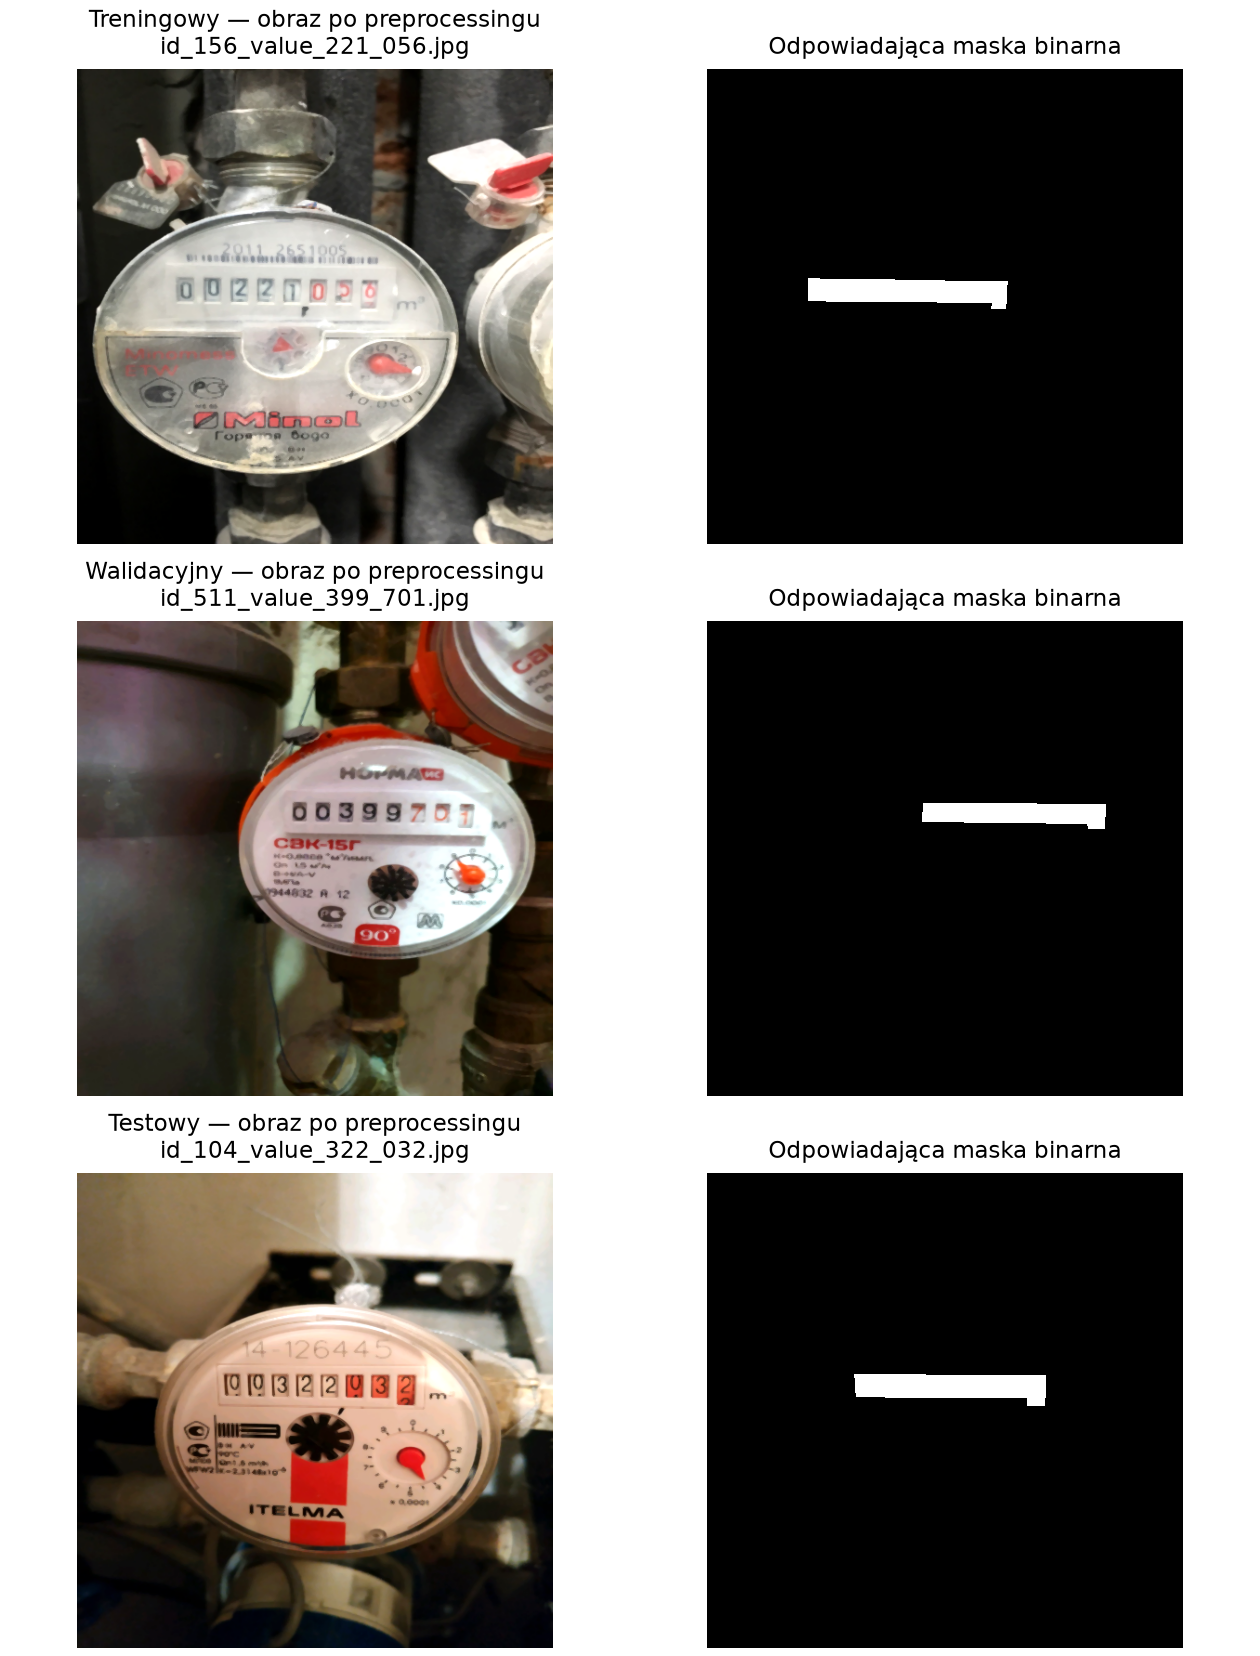
\includegraphics[height=0.58\textheight,keepaspectratio]{preprocessing_examples.png}

\small Przykładowe pary z~każdego podzbioru: po lewej obraz po preprocessingu,
po prawej odpowiadająca mu maska referencyjna. Biały obszar oznacza miejsce
odczytu. Przykłady nie zawierają losowej augmentacji.
\end{center}

\section{Założenia rozwiązania}

Podstawą rozwiązania jest sieć konwolucyjna U-Net w~bibliotece PyTorch,
z~czterema poziomami kodera, podwójnymi blokami konwolucyjnymi i~16 filtrami
w~pierwszym bloku. Połączenia między koderem i~dekoderem pomagają zachować
informację o~położeniu obszaru odczytu.

Docelowe narzędzie powinno przyjmować zdjęcie, wyznaczać maskę oraz umożliwiać
zapis wyniku i~podgląd maski nałożonej na obraz.

\newpage

\section{Hipotezy i plan eksperymentów}

Porównanie obejmie trzy warianty tej samej architektury. Pozwoli to ocenić
wpływ augmentacji bez jednoczesnej zmiany budowy sieci.

\begin{center}
\renewcommand{\arraystretch}{1.18}
\begin{tabularx}{\linewidth}{@{}lY@{}}
\toprule
\textbf{Wariant} & \textbf{Przygotowanie danych treningowych} \\
\midrule
A — baseline & Podstawowe przetwarzanie, bez losowej augmentacji; punkt odniesienia. \\
B & Jak w~A, dodatkowo odbicia poziome i~pionowe oraz obroty do $\pm10^\circ$. \\
C & Jak w~B, dodatkowo losowa zmiana jasności o~maksymalnie 20\%. \\
\bottomrule
\end{tabularx}
\end{center}

\textbf{Hipoteza H1:} wariant B uzyska wyższy średni Dice na zbiorze
walidacyjnym niż wariant A.

\textbf{Hipoteza H2:} wariant C uzyska wyższy średni Dice na zbiorze
walidacyjnym niż wariant B.

Przekształcenia geometryczne będą identyczne dla zdjęcia i~maski;
zmiana jasności dotyczy tylko zdjęcia. Augmentacja obejmie wyłącznie trening.

Warunki porównania będą wspólne: ten sam podział danych, rozdzielczość,
architektura i~ustalone ziarna losowe. Przyjęto funkcję straty
\texttt{BCEWithLogitsLoss}, optymalizator Adam z~learning rate $10^{-4}$
i~\texttt{weight decay} $10^{-4}$ oraz batch size równy 4. Limit treningu
wyniesie 100 epok, z~redukcją learning rate przy zastoju i~zatrzymaniem
po 5 epokach bez poprawy straty walidacyjnej.

Dla każdego wariantu zostanie zapisany checkpoint o~najniższej stracie
walidacyjnej. Następnie warianty zostaną porównane według średniego Dice
na walidacji. W~planowanym porównaniu wyniki testowe nie będą służyć
do strojenia parametrów ani wyboru wariantu. Końcowy test zostanie wykonany
po wczytaniu wag wybranego checkpointu. Zestawienie wyników będzie zawierać
konfigurację, liczbę epok i~metryki. Pojedyncze przebiegi dadzą ocenę wstępną;
małych różnic nie należy traktować jako rozstrzygających bez powtórzeń.

\section{Metryki i kryteria oceny}

\begin{itemize}
  \item \textbf{Dice} — główna metryka, określająca zgodność przewidzianego
  obszaru z~maską referencyjną. Posłuży do porównania wariantów.
  \item \textbf{IoU} — udział części wspólnej predykcji i~maski w~ich sumie;
  uzupełni ocenę pokrycia obszaru odczytu.
  \item \textbf{Odległość Hausdorffa} — dodatkowa miara rozbieżności
  przestrzennej masek, wyrażona w~pikselach przy rozdzielczości $512\times512$.
  \item \textbf{Dokładność pikselowa} — miara pomocnicza, interpretowana
  z~uwzględnieniem dużego udziału tła.
\end{itemize}

Metryki będą liczone dla poszczególnych zdjęć i~uśredniane dla zbioru.
Roboczym celem jakościowym jest średni Dice co najmniej 0,85 na teście.
Jest to przyjęte kryterium projektu, a~nie uniwersalny próg użyteczności.
Ocenę uzupełni przegląd najlepszych i~najgorszych predykcji oraz opis błędów,
np. pominięcia obszaru odczytu lub zaznaczenia fragmentu tła.

W~końcowym etapie planowana jest warstwa XAI oparta na zasłanianiu kolejnych
fragmentów zdjęcia i~pomiarze zmiany odpowiedzi modelu w~ustalonym obszarze
odczytu. Powstała mapa wpływu pomoże sprawdzić, czy predykcja zależy głównie
od tego obszaru, czy również od otoczenia. Będzie to uzupełnienie metryk
i~analizy błędów.

\end{document}
